\documentclass[twoside=false,DIV=14]{scrartcl}

\usepackage{arev} % order matters, putting this above allows FiraSans to override it for body text
\usepackage[sfdefault]{FiraSans}
\usepackage{inconsolata}
%\usepackage[fira]{fontsetup}
\usepackage{scrlayer-scrpage}
\renewcommand{\titlepagestyle}{scrheadings}
\usepackage{graphicx}
\usepackage{blindtext}
\usepackage{wrapfig}
\usepackage{tabularx}
\usepackage{hyperref}
\usepackage{listings}
\usepackage{tikz}
\usepackage{amsmath}
\usepackage[many]{tcolorbox}

\usepackage{xcolor,sectsty}
\definecolor{blackish}{RGB}{56,58,54}
\definecolor{redish}{RGB}{109,41,49}
\definecolor{red}{RGB}{152,41,50}
\definecolor{orangeish}{RGB}{188,71,0}
\definecolor{blueish}{RGB}{25,33,139}
\subsubsectionfont{\color{blackish}}
\subsectionfont{\color{blackish}}
\sectionfont{\color{blackish}}

\lohead{\color{red} COMP3000 Programming Languages}
\rohead{
\includegraphics[width=0.5cm]{../logo.jpg}}

\setkomafont{author}{\sffamily \small}
\setkomafont{date}{\sffamily \small}

\DeclareOldFontCommand{\bf}{\normalfont\bfseries}{\mathbf}
\DeclareOldFontCommand{\tt}{\normalfont\ttfamily}{\texttt}

\lstset{basicstyle=\ttfamily}


\date{}
\newtcolorbox{aside}[1][]{
  title=Aside,
  width=0.3\textwidth,
  fonttitle=\bfseries,
  breakable,
  fonttitle=\bfseries\color{black},
  colframe=blueish!80,
  colback=blueish!2
  #1}

\newtcolorbox{note}[1][]{
  title=Note,
  width=\textwidth,
  fonttitle=\bfseries,
  breakable,
  fonttitle=\bfseries\color{black},
  colframe=orangeish!80,
  colback=orangeish!2
  #1}

\newtcolorbox{hint}[1][]{
    title=Hint,
    width=\textwidth,
    fonttitle=\bfseries,
    breakable,
    fonttitle=\bfseries\color{white},
    colframe=blueish!80,
    colback=blueish!2
    #1}

\newtcolorbox{todo}[1][]{
  title=!! TODO !!,
  width=\textwidth,
  fonttitle=\bfseries,
  breakable,
  fonttitle=\bfseries\color{white},
  colframe=red!80,
  colback=red!2
  #1}
  
\providecommand{\tightlist}{%
  \setlength{\itemsep}{0pt}\setlength{\parskip}{0pt}}

\usepackage{amssymb}

\usepackage{listings}
\lstset{basicstyle=\ttfamily}

\title{\color{redish} \vspace{-2em}Assignment One: The last datatype on earth}

\begin{document}
{\color{blackish}\maketitle}\vspace{-2em}
\begin{abstract}
    A villain has come to Java city and they have wiped out all the integers!  They also wiped out all the value types (\lstinline{boolean}, \lstinline{float}, \lstinline{double}, \lstinline{byte}, etc).  They've promised to come after the java standard library and any reference types next.
\end{abstract}

\begin{wrapfigure}{r}{0.45\textwidth} %this figure will be at the right
  \centering
  
\includegraphics[width=0.45\textwidth]{villain.jpeg}
\end{wrapfigure}

\section{Introduction}
Your task is to start rebuilding civilisation by creating a \lstinline{Church} class which can work just like the integers we lost.  It should have the following functionality:
\begin{itemize}
  \item The integer zero is represented as \verb|null|.
  \item You can make a \lstinline{Church} representing one
  \item You can make a \verb|Church| from any other Church.  It will represent the number one more than the \verb|Church| it was built from.
  \item You can perform simple arithmetic (add, subtract, and multiply) with \lstinline{Church} objects.
\end{itemize}

\section{Starting Point}
Your trusty side-kick Graal has created a class with the right method signatures to get you started. Graal also creates a test file which tests the basics of the \verb+Church+ data type/class. You will find these in the \lstinline{Graal.zip} file on iLearn.\footnote{Thanks to Microsoft CoPilot for our imagery.}


\section{Your task}
Complete the \lstinline{Church} class so that it passes all the tests written by Graal and matches the specification given below.  To avoid being vaporised by the villain \emph{you must not}:
\begin{itemize}
\item Import any libraries
\item Use any integers, doubles, floats, boolean, or any other types at all.
\item Use \verb+String+s.
\item Use any other classes or types at all.
\end{itemize}
You have access to all the control flow, the \lstinline{Church} class, and nulls.

\section{Specifications}

Rules
\begin{itemize}
 \item Minimum JDK version: JDK 8
 \item You must attempt the methods in \lstinline{src/Church.java}
 \item You must pass the tests provided in \lstinline{src/tests/ChurchTest.java}
 \item You should not hard-code your implementations to these tests cases,
additional test cases will be used for marking that are trivial for a
valid implementation.
 \item You may add your own tests to these files, noting that test files are
not submitted
\end{itemize}

The \lstinline{Church} class must implement the following methods (Graal has created the method signatures for you).
\begin{description}
\item [constructors] There should be two constructors.  One takes no arguments and sets up the object to represent the number one.  The other takes a \emph{smaller} \lstinline{Church} and represents the number one larger than the smaller \lstinline{Church}.
\item [equals] Graal has created an equals to override the built-in one and work with tests, but it needs you to complete the more specific \verb|public boolean spec_equals(Church o)| version to work properly.  I can tell you that basically none of your tests will pass without this method so make it your priority.  Graal snuck the last few \verb+boolean+s they could scrounge up just for this purpose.  We have chosen to risk it with these in our test file.  We will destroy the test file if it gets detected.
\item [incr] Returns a \verb|Church| which represents the number one larger than \verb|this|.
\item [decr]  returns a \verb|Church| which represents the number one smaller than \verb|this|.  If the number already represented 1, then it goes to zero (\verb+null+).  You can't decrement zero,  attempting to do so should give a null pointer exception.
\item [plus] A method which takes one argument, the \lstinline{other} \lstinline{Church} which is added to \lstinline{this} \lstinline{Church}. returns a \verb|Church| which represents the number resulting from the addition.
\item [minus] A method which takes one argument - the \lstinline{other} \lstinline{Church} - which is subtracted from \lstinline{this} \lstinline{Church}. Returns a \verb|Church| which represents the number resulting from the subtraction.  If the second number is greater than or equal the first (i.e. the result should be zero or negative), the result should be zero (i.e. \verb+null+).
\item [mult]A method which takes one argument, the \lstinline{other} \lstinline{Church} which is multiplied to \lstinline{this} \lstinline{Church}. Returns a \verb|Church| which represents the number resulting from the multiplication.
\end{description}

Submission requirements
\begin{itemize}
  \item You must submit ONLY your \lstinline{Church.java} file to the ilearn assignment 1 submission box.
  \item Do not rename the submitted file, it must be named \lstinline{Church.java} as provided in the starting template.
  \item Your \lstinline{Church.java} file must compile. If you see any compilation errors prior to submission, you must fix them. These will show:
  \item You must NOT make use of any Java standard library packages, classes, or objects. You cannot create equivalents either.
  \item You must not be at risk of vapourisation by the villain.
\end{itemize}
Recommendation: Once you have submitted, redownload your submitted file
and ensure it is the file you intended to submit. It is worth double-checking by re-running it against the tests and checking if the result is as you expect

\section{Hints}
This assignment tests  your understanding of, and ability to code, \emph{recursive data types} like the linked list we looked at in lectures.  Your solution \emph{will need to be a recursive data type very much like that linked list}.  You may need to use some imagination to see the similarity, but when you see it, all will be revealed\footnote{The ability to find \emph{isomorphisms} is your superpower, use it to save Java city}.

\begin{wrapfigure}{l}{0.35\textwidth} %this figure will be at the right
  \centering
  
\includegraphics[width=0.35\textwidth]{graal.jpg}
\end{wrapfigure}


\subsection{Still don't get it?}
There will be a discussion in the lecture in week 3.  You should watch (and rewatch) that discussion.  You should discuss the discussion with your classmates and your tutor.  You should write out your understanding of the discussion.  If you are still confused after going through these steps, email Matt with a copy of what you wrote up and he will organise a chat to help.

\subsection{Tips}
You will find the work easier if you write a \verb+toString()+ method for your \verb+Church+ class.  However, this involves using \verb+String+s which is not allowed!  \emph{If} you want to go down this route to help you during your development, be sure to triple check you have removed any sign of \verb+String+s before you submit your code or your grades could get vapourised.

\section{Bonus}
Get extra chances at the lecture prize draw by posting your thoughts regarding why Graal has called the class \lstinline{Church} to the unit Forum.  There are also extra chances up for grabs for coming up with a good name for our villain or for ourselves (the hero).

\section{Grading}
Your submitted file will be run against a test program consisting of the tests Graal delivered to you and an additional 6 tests.  Passing each test is worth marks according to the following table.  Note, you will not be given the test script for the additional tests but can guess what they do from the names

\begin{tabular}{lcl}
  \textbf{test name} & \textbf{provided by Graal} & \textbf{value} \\
  \hline
  testEqualsDirectly & $\checkmark$ & 5 \\
  testEqualsIndirectly & & 5 \\
  testIncr & $\checkmark$ & 5 \\
  testIncrTwo & & 5 \\
  testDecr & $\checkmark$ & 5 \\
  testDecrTwo & & 5 \\
  testPlus & $\checkmark$ & 5 \\
  testPlusTwo & & 5 \\
  testMinus & $\checkmark$ & 5 \\
  testMinusTwo & & 5 \\
  testMult & $\checkmark$ & 5 \\
  testMultViaEverything & & 10 \\
  \hline
  \hline
  total & & 65 \\
  \hline
\end{tabular}
\vspace{2em}

The following penalties will apply on top of that rubric:

\begin{tabular}{ll}
\textbf{error} & \textbf{penalty} \\
\hline
Use of value type & -30 \\
Use of String & -30 \\
Failure to compile & -65 \\
Importing anything & -20 \\
Risk of vapourisation & -30 \\
Submitting a solution generated by someone or something else & -65 \\
\end{tabular}

\newpage
\section{Solution}

The key to solving this problem is to notice that the description given of \lstinline{Church} is very similar to the description of a linked list.  In fact, the \lstinline{Church} class \emph{is} a linked list but one that does not need to store any values.  The length of the list has all the information that is needed.  Thus we end up writing \lstinline{Church} just the same as a linked list

\begin{lstlisting}[language=java]
  public class Church {
    Church smaller;
    
    public Church(){
      smaller = null;
    }
    
    public Church(Church from){
      smaller = from;
    }
\end{lstlisting}

The \lstinline{Church} class only needs a single field to point to the smaller \lstinline{Church} object.  We create two constructors.  The first is for constructing the \lstinline{Church} representing one, the other represents a \lstinline{Church} one larger than the one it was given.

Notice that this makes it impossible to create a \lstinline{Church} object representing zero. This is generally a problem in programming, how to represent different types of \emph{nothingness}.  The general solution in Java is to use \lstinline{null} to represent zero.  We can also use \lstinline{null} to represent the end of the list\footnote{Which is perfect because the number one less than one is zero!}.  This is an interesting property of recursive data in Java, there is no way to represent the \emph{empty} data within the class itself, you always need to use \lstinline{null}.

\lstinline{incr} and \lstinline{decr} are simple functions with no looping or recursion needed
\begin{lstlisting}[language=java]
  public Church incr(){
    return new Church(this);
  }

  public Church decr(){
    return smaller;
  }
\end{lstlisting}

Recursive solutions are by far the simplest for the others, so we will provide them.

You will notice we need to take care of the cases where the \lstinline{other} \lstinline{Church} is null (representing zero) specifically, and then also need to deal with the case of \lstinline{one} because it won't have a smaller \lstinline{Church} within it.  With those two cases dealt with, the functions are all recursive.  Adding two numbers is the same as adding one less then incrementing.  Multiplying two numbers is the same as adding once, then multiplying one less.  Subtracting two numbers is the same as subtracting one less from one less.
\begin{align*}
  a + b & = a + (b - 1) + 1 \\
  a \times b & = a + (a \times (b - 1)) \\
  a - b & = (a - 1) - (b - 1)
\end{align*}


\begin{lstlisting}[language=java]
  public Church plus(Church other){
    if (other == null){
        return this;
    } else {
        return plus(other.smaller).incr();
    }
  }

  public Church mult(Church other){
    if (other == null)
        return null;
    if (other.smaller == null)
        return this;
    if (smaller == null)
        return other;
    else{
        return mult(other.smaller).plus(this);
    }
  }

  public Church minus(Church other){
    if (smaller == null && other != null){
        return null;
    } else if (other == null){
      return this;
    } else {
        return smaller.minus(other.smaller);
    }
  }
\end{lstlisting}

\subsection{Dealing with equality}
We need equality for the testing.  This is a hassle and we would prefer to leave it out, but we can't test without it.  The specification tells us that Graal has snuck in the last available booleans, which you can see here

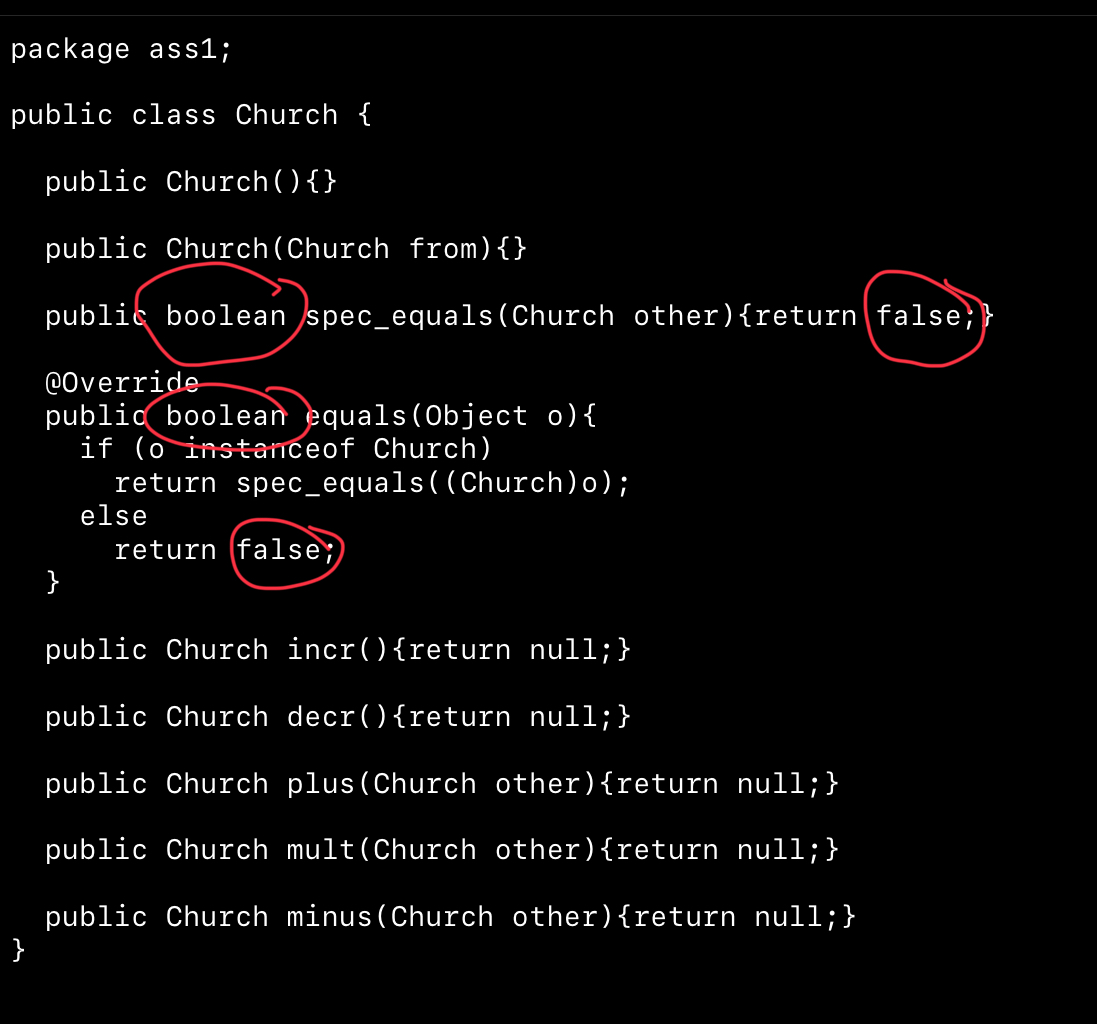
\includegraphics[width=0.5\textwidth]{last_booleans.jpeg}

It is clear from the specification that \emph{we should do everything we can not to introduce any more booleans!} so we will keep this in mind as we generate our solution.

We only need to fill in \lstinline{spec_equals}, which is comparing this \lstinline{Church} to another.  Two \lstinline{Church}s are the same if: \begin{itemize}
  \item they are both \lstinline{null} (zero) or
  \item they are both \lstinline{Church} objects and their smaller \lstinline{Church} objects are equal
\end{itemize}
The first condition is encoded as
\begin{lstlisting}[language=java]
  if (this == null && o == null)
    return true;
\end{lstlisting}
\emph{but} I don't want to introduce that extra boolean literal!  In this situation we can use the old trick\footnote{COMP1000} where returning \lstinline|true| is the same as returning the condition itself, so I could write it as
\begin{lstlisting}[language=java]
  return this == null && o == null;
\end{lstlisting}
Once I apply the same trick with the other condition, the answer for \lstinline{spec_equals} is
\begin{lstlisting}[language=java]
  public boolean spec_equals(Church o){
    return (this == null && o == null) || smaller.spec_equals(o.smaller);
  }
\end{lstlisting}
We even managed to remove a boolean, good for us!  It is a fun puzzle to work through from the first solution to one that avoids vapourisation.

\end{document}

